\documentclass{article}
\usepackage{amsmath, amssymb, mdwlist, graphicx, hyperref}
\usepackage{listings,color}
\usepackage{wrapfig}
\usepackage[usenames,dvipsnames]{xcolor}
\definecolor{gray}{rgb}{0.97,0.97,0.97}
\lstset{%
language=C,%
%backgroundcolor=\color{gray},
emph={putpixel},
emphstyle=\bf,
tabsize=4,
framesep=5pt,
mathescape=true,
xleftmargin=0.1cm,
xrightmargin=0.1cm,
frame=lines,
%basicstyle=\ttfamily,
%keywordstyle=\color{Blue},
%commentstyle=\color{OliveGreen},
%stringstyle=\color{MidnightBlue},
columns=flexible,
%showstringspaces=false
}

\newcommand{\mpar}[1]{\marginpar{\textit{#1}}}
\newcommand{\norm}[1]{\Vert #1 \Vert}
\DeclareMathOperator{\argmax}{argmax}
\DeclareMathOperator{\argmin}{argmin}
\newenvironment{solution}{\paragraph{Solution.}$\,$ }{\vskip 3mm\hrule}
\newenvironment{exercise}[2]{\paragraph{Exercise #1 (#2pt).} }{
\medskip}
\newcommand{\bbR}{\mathbb{R}}
\newcommand{\bw}{\mathbf{w}}
\newcommand{\bx}{\mathbf{x}}
\newcommand{\bd}{\mathbf{d}}
\newcommand{\bb}{\mathbf{b}}
\newcommand{\by}{\mathbf{y}}
\newcommand{\bzero}{\mathbf{0}}
\newcommand{\bz}{\mathbf{z}}
\newcommand{\bSigma}{\mathbf{\Sigma}}
\newcommand{\bp}{\mathbf{p}}
\newcommand{\bP}{\mathbf{P}}
\newcommand{\bm}{\mathbf{m}}
\newcommand{\bc}{\mathbf{c}}
\newcommand{\bM}{\mathbf{M}}
\newcommand{\bV}{\mathbf{V}}
\newcommand{\bK}{\mathbf{K}}
\newcommand{\bD}{\mathbf{D}}
\newcommand{\bA}{\mathbf{A}}
\newcommand{\bX}{\mathbf{X}}
\newcommand{\bY}{\mathbf{Y}}
\newcommand{\bR}{\mathbf{R}}
\newcommand{\bI}{\mathbf{I}}
\newcommand{\bS}{\mathbf{S}}
\newcommand{\bT}{\mathbf{T}}
\newcommand{\balpha}{\boldsymbol{\alpha}}
\newcommand{\pt}[2]{\left(\begin{array}{c}#1\\#2\end{array}\right)}

\begin{document}
\title{MTAT.03.015 Computer Graphics (Fall 2013)\\
Exercise session X: OpenGL 3.1+}
\author{Konstantin Tretyakov, Ilya Kuzovkin}
\date{November 11, 2013}
\maketitle

In this exercise session we shall study the specifics of OpenGL beyond version 3.1 -- something we have been delaying for as much as possible in order to keep things simple. As usual, the base code is provided in the \texttt{practice10.zip} archive on the course website or via the course github page. Download, unpack and open it. You will need to submit your solution as a zipped archive file.

\section{OpenGL Beyond 3.1}
OpenGL ideology changed significantly at around version 3.1. Starting from that version, most of the functions that we have been actively using in the previous exercise sessions were deprecated and removed. This includes:
\begin{enumerate}
\item Default vertex and fragment processing. Modern OpenGL provides absolutely no defaults and requires you to fully specify the logic of vertex and fragment shaders. There is no \texttt{ftransform} any more, nor are there any of the convenient built-in state variables, such as \verb#gl_Vertex#, \verb#gl_ModelViewMatrix#, or \verb#gl_LightSource[]#.
\item Consequently, everything that has to do with specifying parameters for default lighting and texture mapping computations (\texttt{glLight}, \texttt{glTexCoord}, \texttt{glTexGen}, \texttt{glTexEnv}) is not part of modern OpenGL. If you want to do lighting or texture mapping, you have all the freedom in the shaders. You can pass all the necessary parameters as shader uniform variables.
\item The matrix stack has also been removed, i.e. you cannot use \texttt{glLoadIdentity}, \texttt{glPushMatrix}, \texttt{glRotate}, etc. With custom shaders you are free to prepare a matrix to your liking and pass it as a uniform, if you want.
\item Finally, triangle specification using \texttt{glBegin}, \texttt{glEnd} and \texttt{glVertex} is also gone. Sending vertex coordinates from the application to the graphics card \emph{every time} you need to draw a triangle, making a separate function call for each vertex, is very inefficient. Things become worse if you need to draw millions of triangles, and those are the same triangles every frame. A much better way is to upload a whole array of data to the GPU once, and then use a single function call to request the GPU to render vertices from that array. In the old OpenGL this was an option. In the modern version this is the only way to go.
\end{enumerate}

At this point you might feel like absolutely everything you knew about OpenGL so far disappeared in 3.1. This is not true, though. The gist of the change is quite simple: there are no defaults any more, so you have to use shaders, and there is no \texttt{glBegin} and \texttt{glEnd}, so you have to use \emph{vertex array objects}.

If at any point you might be wondering which functions are available in which versions, the easiest option is to consult the OpenGL manual pages for version 2.1\footnote{\url{http://www.opengl.org/sdk/docs/man2/}}, 3.3\footnote{\url{http://www.opengl.org/sdk/docs/man3/}} and 4\footnote{\url{http://www.opengl.org/sdk/docs/man4/}}. The history page\footnote{\url{http://www.opengl.org/wiki/History_of_OpenGL}} on the OpenGL Wiki provides a convenient high-level changelog.

\begin{exercise}{1}{1.5}
Open the project \verb#1_NewTriangle# and study the code. You will see the familiar GLUT application structure. Some things are worth paying special attention to, however:
\begin{enumerate}
\item First take note of the lines
\begin{verbatim}
  glutInitContextVersion(3, 3);
  glutInitContextProfile(GLUT_CORE_PROFILE);
\end{verbatim}
Those lines request GLUT to ensure that OpenGL would follow the version 3.3 \emph{core profile} specification. Since the introduction of backward-incompatible changes many graphics card vendors decided to still keep the old functions around. Hence, to distinguish between ``strict 3.3'' mode and ``let's  have the older functions around'' mode, the notion of \emph{core} and \emph{compatibility} profiles was introduced. Requesting \verb#GLUT_COMPATIBILITY_PROFILE# will let you (in most cases\footnote{Mac is the main example, that does not support the compatibility profile.}) use the old functions alongside the new ones. Requesting the core profile declares your commitment to strictly follow the newer specifications.

Version 3.3 of OpenGL is the last version before OpenGL 4 and is probably the best choice for practicing the ``new style'', as OpenGL 4 is not as widely supported yet. The corresponding GLSL version is also 3.3.

\item Secondly, study the function \verb#prepare_vertex_data#. As noted above, in the newer OpenGL the vertices are not specified by giving their coordinates via \texttt{glVertex} any more. Instead, you are free to feed any kind of data to define the vertices. For example, you could say that each vertex is defined by a single integer, and use the vertex shader to convert this integer into actual position somehow\footnote{In fact, each vertex \emph{is} identified by an integer named \texttt{gl\textunderscore VertexID} in the shader.}. Or you could be more conventional and say that each vertex has three attributes: its position, normal and color, etc.

The information on which attributes will be passed for each vertex is stored in a \emph{vertex array object}. The object is created using the \texttt{glGenVertexArrays} call. This call returns a \emph{handle} to the created object. You can then \emph{bind} this handle to be the ``currently active vertex array'' using \texttt{glBindVertexArray}. You have already seen similar logic when operating with textures: you create them using \texttt{glGenTextures} and you ``make them currently active'' using \texttt{glBindTexture}.

Besides the vertex array, another object is created in \verb#prepare_vertex_data# -- an \emph{array buffer}. The creation logic is again the same: \texttt{glGenBuffers} followed by \texttt{glBindBuffer}.

What happens further is the following: we upload a bunch of floating point numbers from \texttt{vertexData} into the created buffer (note that this corresponds to transferring the data to the GPU). Next we add an attribute (numbered 0) to our vertex array object, and specify how the values for this attribute should be read from the array buffer.

Once we have done it, we can use this attribute in the vertex shader by writing
\begin{verbatim}
  layout(location = 0) in vec2 position;
\end{verbatim}

Finally, the actual rendering is happening using a single call: \texttt{glDrawArrays}. This call is equivalent to invoking \texttt{glBegin}, emitting a number of vertices (each with its accompanying attributes) from the vertex array, and closing with a \texttt{glEnd}.

\item The line
\begin{verbatim}
   glBindFragDataLocation(shader, 0, "fragColor");
\end{verbatim}
specifies the name of the output variable of the fragment shader (essentially defining what will be acting as \verb#gl_FragColor#).


\item The line 
\begin{verbatim}
  #include <glutil/MatrixStack.h>
\end{verbatim}
lets us use the implementation of the matrix stack from the \emph{GL Util} library\footnote{\url{http://glsdk.sourceforge.net/docs/html/classglutil_1_1_matrix_stack.html}}. It also implicitly includes the \emph{GLM matrix library}\footnote{\url{http://glm.g-truc.net/0.9.4/api/modules.html}}.


\item The \texttt{display} function makes use of the MatrixStack class to prepare a matrix and send it to the shader as a uniform variable.
\end{enumerate}
Make sure you understand everything that is happening here. Your task in this exercise consists of two parts:
\begin{enumerate}
\item Add a \emph{color} attribute to each vertex. Make one vertex red, another green and the third one blue. For that you will need to modify the \texttt{vertexData} array, change the existing \texttt{glVertexAttribPointer} call, add another \texttt{glEnableVertexAttribArray} accompanied with its own\\ \texttt{glVertexAttribPointer}, change the vertex shader and the fragment shader a bit.
\item Render a smaller (scaled by 0.3) rotating copy of the triangle centered at position (0.5, 0.5). Use the \texttt{Push} and \texttt{Pop} methods of the \texttt{MatrixStack} object if needed.
\end{enumerate}

The result could look as follows:
\begin{center}
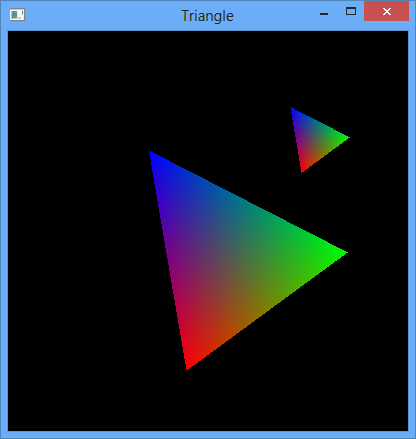
\includegraphics[width=0.7\textwidth]{newtriangle.png}
\end{center}
\end{exercise}

\begin{exercise}{2}{1}
Add a second scene\footnote{There is a \texttt{current\textunderscore scene\textunderscore id} variable that changes its value when the \emph{Space} or \emph{Return} key is pressed. Use an \texttt{if (current\textunderscore scene\textunderscore id == ..)} condition in the \texttt{display} function.} to the project, that would render a simple rotating cube with colored faces. For that:
\begin{enumerate}
\item Create a second vertex array object with its own vertex coordinates and colors, appropriate for the cube. Ensure that each face has its own solid color (for that you will need to repeat vertices, i.e. you will have a total of 24 vertices in the array).
\item You will need to modify the first vertex array and the shader to use three-dimensional vertices (rather than two-dimensional).
\item In the \texttt{display} function you will have to select which vertex array to use by calling \texttt{glBindVertexArray} with the appropriate handle.
\item Do not forget to use perspective projection (\texttt{MatrixStack::Perspective}) and set an appropriate view transform. As you have no lighting computations, you do not need to keep separate matrices for model-view and projection -- the existing \texttt{modelViewProjectiomMatrix} uniform variable will suffice.
\item Finally, use 6 calls to \verb#glDrawArrays# -- one for each face. You will need to use either \verb#GL_TRIANGLE_FAN# or \verb#GL_TRIANGLE_STRIP# primitive type, depending on which order you listed the vertices for each face.
\end{enumerate}
\end{exercise}

\begin{exercise}{3*}{0.5}
Modify the last exercise to use a single call to \verb#glDrawElements# rather than six calls to \verb#glDrawArrays#. For that you will need to create another buffer object, bind it to the \verb#GL_ELEMENT_ARRAY_BUFFER# target, and fill with a sequence of integers. Read this\footnote{\url{http://www.opengl-tutorial.org/intermediate-tutorials/tutorial-9-vbo-indexing/}} for explanations.
\end{exercise}

\section{WebGL and OpenGL ES*}
\begin{exercise}{4*}{1.5}
WebGL is an OpenGL specification tuned for the Web browser. In spirit it is quite close to OpenGL 3.1, so it is not too hard to port the code you just wrote to WebGL (only the matrix library and the shader utility class may significantly differ). Study an introductory WebGL tutorial\footnote{\url{http://learningwebgl.com/blog/?p=28} should be enough, but you are welcome to google for more}, and port any of the two scenes you just implemented (or both, if you wish) to run in the browser.
\end{exercise}

\begin{exercise}{5*}{0.5}
Implement a rotating colored cube scene in the browser using the Three.js\footnote{\url{http://threejs.org/}} library.
\end{exercise}

\begin{exercise}{6* [Deadline: December 1]}{1.0}
Port the two-scene application from Exercise 2 to run on Android. Android phones run a version of OpenGL API called OpenGL ES. Like WebGL, OpenGL ES (at least starting from version 2.0) largely follows the OpenGL 3.1+ specification.

You can attempt this task in two ways. The first and the most obvious approach is to use the native Android development tools and port the code to Java\footnote{\url{http://developer.android.com/guide/topics/graphics/opengl.html}}.

Another approach is to use the fact that the bleeding-edge version of FreeGLUT lets you compile GLUT applications directly for Android. The steps necessary to compile for Android are described on the FreeGLUT website\footnote{\url{http://freeglut.sourceforge.net/docs/android.php}}. There is also a sample project in the FreeGLUT source code in the SVN repository (NB: it is \emph{not} present in the zipped archive you can download from the website, you must checkout from SVN). 

The deadline for this exercise is December 1. Note: it only makes sense to attempt this task if you have some experience with Android development, or are comfortable with following cross-compilation instructions like those given on the FreeGLUT website, debugging the issues that come up on the way. The point count for this task is 1 not because it is necessarily ``easy''\footnote{It is not technically hard, but it can be very time-consuming if you manage to stumble into an unexpected debugging hole.}, but simply because the skills and equipment it requires are not a prerequisite for this course.

If you are an Apple or a Windows phone user, you are welcome to try porting the application to your device instead. However, I won't be able to consult you much if you get into problems on those platforms. In this case, in addition to submitting the project code you should also demonstrate in person that the project works on your device.
\end{exercise}

\end{document}
